\documentclass[uplatex,11pt]{jsarticle}
\usepackage[dvipdfmx]{graphicx}
\usepackage{url}

% タイトル・著者情報の決定
\title{日本におけるデジタル化の状況}
\author{G684652026 鈴木 爽太}
\date{2026年7月6日}

\begin{document}

\maketitle

\section{ブロードバンドの整備状況}
OECDによるブロードバンド回線の普及に関する調査\cite{oecd2022}によると，図\ref{fig:broadband}に示すように，日本における100人あたりのモバイルブロードバンドの加入者数は 190.5 で，第1位になっている．2位はエストニアで，3位米国と続く．

\begin{figure}[htbp]
    \centering
    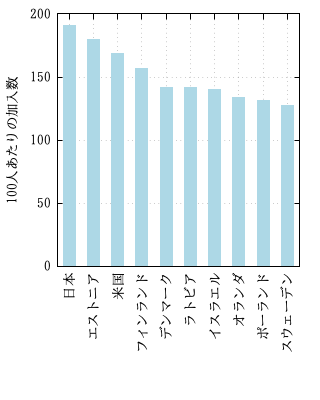
\includegraphics[width=0.45\textwidth]{fig23.png}
    \caption{光ファイバー回線の加入者数（100人あたり）}
    \label{fig:broadband}
\end{figure}

\newpage

\section{デジタル競争力ランキング}
国際経営開発研究所（IMD）の調査\cite{imd2021}によると，日本のデジタル競争力のランキングは表\ref{tab:ranking}に示すように，調査対象の64カ国中，総合で28位，技術分野で30位となっている．

\begin{table}[htbp]
    \centering
    \caption{デジタル競争力ランキング（64カ国中）}
    \label{tab:ranking}
    \begin{tabular}{|c|c|c|}
        \hline
        国 & 総合 & 技術 \\ \hline
        米国 & 1位 & 4位 \\ \hline
        香港 & 2位 & 10位 \\ \hline
        スウェーデン & 3位 & 8位 \\ \hline
        デンマーク & 4位 & 2位 \\ \hline
        シンガポール & 5位 & 3位 \\ \hline\hline
        韓国 & 12位 & 13位 \\ \hline
        中国 & 15位 & 20位 \\ \hline\hline
        日本 & 28位 & 30位 \\ \hline
    \end{tabular}
\end{table}

\section{考察}
\begin{itemize}
    \item 図\ref{fig:broadband}を見ると日本はネットの回線環境が世界1位なのに、表\ref{tab:ranking}のデジタル競争力では28位とかなり低いのがもったいないと感じた。
    \item 日本は最高のネットインフラを持っていながら、それを勉強や仕事、新しい技術開発にうまく活かしきれていないのではないかと思う。
    \item 今後はただ回線の普及率を上げるだけでなく、学校や社会全体でもっとデジタル技術を使いこなせる人を増やしていくことが大切だと考えられる。
\end{itemize}

\vspace{3em}

\begin{thebibliography}{9}
    \bibitem{oecd2022} OECD. Broadband Portal. \url{https://www.oecd.org/digital/broadband/broadband-statistics/}, 2022.
    \bibitem{imd2021} IMD. IMD world digital competitiveness ranking. \url{https://www.imd.org/centers/world-competitiveness-center/rankings/world-digital-competitiveness/}, 2021.
\end{thebibliography}

\end{document}